\tikzset{every picture/.style={line width=0.75pt}} %set default line width to 0.75pt        

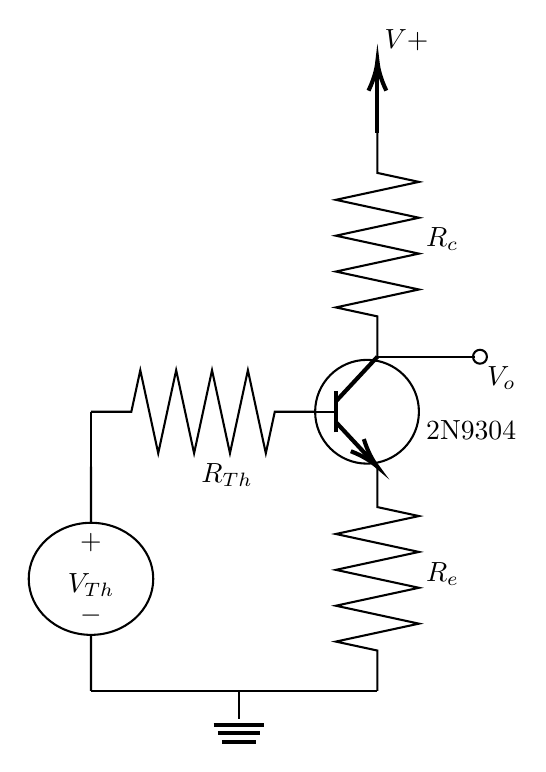
\begin{tikzpicture}[x=0.75pt,y=0.75pt,yscale=-1,xscale=1]
%uncomment if require: \path (0,497); %set diagram left start at 0, and has height of 497

%Shape: Resistor [id:dp5471354453834067] 
\draw   (173.42,205.5) -- (192.86,205.5) -- (197.18,185.5) -- (205.82,225.5) -- (214.46,185.5) -- (223.1,225.5) -- (231.74,185.5) -- (240.38,225.5) -- (249.02,185.5) -- (257.66,225.5) -- (261.98,205.5) -- (281.42,205.5) ;
%Shape: Resistor [id:dp42863709400980965] 
\draw   (311.42,71) -- (311.42,90.44) -- (331.42,94.76) -- (291.42,103.4) -- (331.42,112.04) -- (291.42,120.68) -- (331.42,129.32) -- (291.42,137.96) -- (331.42,146.6) -- (291.42,155.24) -- (311.42,159.56) -- (311.42,179) ;
%Shape: Resistor [id:dp18218903209345216] 
\draw   (311.42,232) -- (311.42,251.44) -- (331.42,255.76) -- (291.42,264.4) -- (331.42,273.04) -- (291.42,281.68) -- (331.42,290.32) -- (291.42,298.96) -- (331.42,307.6) -- (291.42,316.24) -- (311.42,320.56) -- (311.42,340) ;
%Straight Lines [id:da236864146953923] 
\draw    (173.42,205.5) -- (173.42,232) ;
%Shape: Circle [id:dp6263492261348075] 
\draw   (281.42,205.5) .. controls (281.42,191.69) and (292.61,180.5) .. (306.42,180.5) .. controls (320.23,180.5) and (331.42,191.69) .. (331.42,205.5) .. controls (331.42,219.31) and (320.23,230.5) .. (306.42,230.5) .. controls (292.61,230.5) and (281.42,219.31) .. (281.42,205.5) -- cycle ;
%Straight Lines [id:da5434466420085665] 
\draw    (291.42,205.5) -- (281.42,205.5) ;
%Straight Lines [id:da8222789328378522] 
\draw [line width=1.5]    (291.42,215.5) -- (291.42,195.5) ;
%Straight Lines [id:da6868248647799469] 
\draw [line width=1.5]    (291.42,210.5) -- (309.38,229.8) ;
\draw [shift={(311.42,232)}, rotate = 227.07] [color={rgb, 255:red, 0; green, 0; blue, 0 }  ][line width=1.5]    (14.21,-4.28) .. controls (9.04,-1.82) and (4.3,-0.39) .. (0,0) .. controls (4.3,0.39) and (9.04,1.82) .. (14.21,4.28)   ;
%Straight Lines [id:da7170401481045089] 
\draw [line width=1.5]    (311.42,179) -- (291.42,200.5) ;
%Straight Lines [id:da09379764529365986] 
\draw    (311.42,340) -- (173.42,340) ;
%Straight Lines [id:da20374241030260287] 
\draw [line width=1.5]    (311.42,71) -- (311.42,39.58) ;
\draw [shift={(311.42,36.58)}, rotate = 90] [color={rgb, 255:red, 0; green, 0; blue, 0 }  ][line width=1.5]    (14.21,-4.28) .. controls (9.04,-1.82) and (4.3,-0.39) .. (0,0) .. controls (4.3,0.39) and (9.04,1.82) .. (14.21,4.28)   ;
%Straight Lines [id:da7615603326736993] 
\draw    (358.49,179) -- (311.42,179) ;
\draw [shift={(360.84,179)}, rotate = 180] [color={rgb, 255:red, 0; green, 0; blue, 0 }  ][line width=0.75]      (0, 0) circle [x radius= 3.35, y radius= 3.35]   ;
%Straight Lines [id:da09982064594930351] 
\draw [line width=0.75]    (244.71,353.42) -- (244.71,340) ;
%Straight Lines [id:da7825511264162391] 
\draw [line width=1.5]    (232.5,356.42) -- (256.92,356.42) ;
%Straight Lines [id:da8263231613187413] 
\draw [line width=1.5]    (234.5,360.42) -- (254.92,360.42) ;
%Straight Lines [id:da4438946372208784] 
\draw [line width=1.5]    (236.5,364.42) -- (252.92,364.42) ;
%Shape: Output [id:dp833046385605702] 
\draw   (173.42,259) .. controls (189.99,259) and (203.42,271.09) .. (203.42,286) .. controls (203.42,300.91) and (189.99,313) .. (173.42,313) .. controls (156.85,313) and (143.42,300.91) .. (143.42,286) .. controls (143.42,271.09) and (156.85,259) .. (173.42,259) -- cycle (173.42,232) -- (173.42,259) (173.42,340) -- (173.42,313) ;

% Text Node
\draw (313.42,33.18) node [anchor=south west] [inner sep=0.75pt]    {$V+$};
% Text Node
\draw (362.84,182.4) node [anchor=north west][inner sep=0.75pt]    {$V_{o}$};
% Text Node
\draw (333.42,208.5) node [anchor=north west][inner sep=0.75pt]   [align=left] {2N9304};
% Text Node
\draw (333.42,115.44) node [anchor=north west][inner sep=0.75pt]    {$R_{c}$};
% Text Node
\draw (333.42,276.44) node [anchor=north west][inner sep=0.75pt]    {$R_{e}$};
% Text Node
\draw (225.1,228.9) node [anchor=north west][inner sep=0.75pt]    {$R_{Th}$};
% Text Node
\draw (173.42,262.4) node [anchor=north] [inner sep=0.75pt]    {$+$};
% Text Node
\draw (173.42,309.6) node [anchor=south] [inner sep=0.75pt]    {$-$};
% Text Node
\draw (173.49,289.19) node    {$V_{Th}$};


\end{tikzpicture}
